\documentclass[pdftex,a4paper,titlepage,12pt]{scrartcl}
\usepackage[utf8x]{inputenc}
\usepackage[paper=a4paper,includefoot,includehead,left=30mm,right=20mm,top=20mm,bottom=20mm]{geometry}
\usepackage[T1]{fontenc}
\usepackage[pdftex]{graphicx}
\usepackage[ngerman]{babel}
\usepackage{thmbox}
%\usepackage{german}
\usepackage
[colorlinks=true,linkcolor=red,
 anchorcolor=black,citecolor=green,
 pagecolor=red,urlcolor=cyan,backref,]{hyperref}
\usepackage{cite}
\usepackage{url}
\usepackage[german]{varioref}
%\usepackage{booktabs}
\usepackage{array}
%Adds a box around floats
\usepackage{float}
\floatstyle{boxed} 
\restylefloat{figure}

\pagestyle{headings}

\newtheorem[L]{boxedDefinition}{Definition}
\newtheorem{definition}{Definition}

\setcounter{secnumdepth}{3}
\setcounter{tocdepth}{3}

%Scriptsized, vertically and horizontally centered tabular column type
\newcolumntype{s}[1]{>{\scriptsize\centering\arraybackslash}m{#1}}

\title{3D-Tumorvisualisation}
\subtitle{Seminararbeit}
\author{Uli Köhler}
%\institute[EMG]{Ernst-Mach-Gymnasium Haar}
\date{9.~November 2010}

\newcommand{\footnoteremember}[2]{\footnote{#2}\newcounter{#1}\setcounter{#1}{\value{footnote}}}
\newcommand{\footnoterecall}[1]{\footnotemark[\value{#1}]}

%Utility to insert a newline after a paragraph declaration
\newcommand{\paranl}{$~~$\\}
\newcommand{\HRule}{\rule{\linewidth}{0.5mm}}

\begin{document}


\begin{titlepage}
 Ernst-Mach-Gymnasium Haar\hfill Kollegiatenjahrgang 2010/2011
\vspace{4cm}
\begin{center}
  
 \large\textsc{Seminararbeit im W-Seminar \glqq Medizinische Bildgebungsverfahren\grqq}\\[2cm]
 {\fontsize{40}{40}\selectfont \textbf{3D-Tumorvisualisation}}\\[2cm]

 \begin{tabular}{ll}
  \textsc{Verfasser:} & Ulrich Köhler\\
  \textsc{W-Seminar:} & Medizinische Bildgebungsverfahren\\
  \textsc{Kursleiter:} & Ernst Bartels\\[2cm]
 \end{tabular}
\vspace{2cm}

\begin{tabular}[c]{|l|s{38mm}|s{38mm}|s{38mm}|}\hline
& schriftlich, einfache Wertung &\scriptsize mündlich &\scriptsize gesamt\\\hline
Erzielte Note & & &\\\hline
Erzielte Punkte & & &\\\hline
\end{tabular}
\vspace{3cm}

\end{center}

Datum der Abgabe im Kollegstufensekretariat\hfill Unterschrift des Kursleiters
\thispagestyle{empty}

\end{titlepage}


\thispagestyle{empty}\newpage
\tableofcontents\thispagestyle{empty}\newpage
\section{Einleitung}\label{sec:introduction}
In dieser Arbeit sollen Methoden und Algorithmen diskutiert und verglichen werden, die zur dreidimensionalen Visualisierung von Tumoren in Echtzeit dienen. Hierzu werden zuerst in Kapitel \vref{ssec:requirements} nach einer Definition dieses Begriffs die allgemeinen Anforderungen sowie in Kapitel \vref{ssec:applications} Anwendungsmöglichkeiten für solche Systeme dargestellt. Darauf aufbauend werden in Kapitel \vref{ssec:swhwcomparison} reine Softwarealgorithmen\footnote{Algorithmus - Verarbeitungsvorschrift} mit auf spezieller Hardware basierenden Algorithmen verglichen. Kapitel \vref{ssec:volsurfacealgorithms} stellt kurz die in dieser Arbeit beschriebenen Volumenrenderingverfahren Oberflächenrenderingalgorithmen gegenüber. Danach zeigt Kapitel \vref{ssec:platforms} einen Überblick der verfügbaren Plattformen zur Implementierung von Visualisationsalgorithmen. Kapitel \vref{ssec:algoexample} führt einen beispielhaften Algorithmus zur Hervorhebung von Tumoren sowie dessen im Rahmen dieser Arbeit entstandene Implementation (\glqq VERTEBRA\footnote{VERTEBRA - Volumetric Examiner for Radiological/Tomographical Experimental Basic Realtime Analysis}\grqq) ein.

Anschließend wird in Kapitel \vref{sec:augmentedreality} das Konzept der \glqq Augmented Reality\grqq\ diskutiert, das bereits jetzt für viele medizinische Visualisationssysteme eingesetzt wird. Mit ARION\texttrademark\  wird in Kapitel \vref{sec:arion} ein Beispiel für ein solches System diskutiert.
Mit dem Schlussteil, der in Kurzform die wichtigsten Thesen, Konzepte und Resultate rekapituliert, endet der Hauptteil dieser Arbeit.
\section{Echtzeit-Tumorvisualisationssysteme}\label{sec:vissystems}
\subsection{Anforderungen}\label{ssec:requirements}
Um die Anforderungen für Echtzeit-Tumorvisualisationssysteme zu erläutern, muss der Begriff zuerst mit allen zu erfüllenden Anforderungen definiert werden. Die folgende Definition basiert auf \cite[Kapitel 3.1.1, Seite 17]{Bruckner2004} sowie auf \cite{Kutter2008}
\begin{boxedDefinition}[Echtzeit-Tumorvisualisationssystem]\label{def:rttumorvissystem}
 Als Echtzeit-Tumorvisualisationssystem sei ein System definiert, das in Echtzeit in der Lage ist, aus dreidimensionalen medizinischen Eingabedatensätzen hochqualitative Ausgabedaten zu generieren, die auf Displays\footnote{Ein Display sei in diesem Kontext ein Gerät, das dazu dient, Informationen visuell anzuzeigen} in ein Weise dargestellt werden können, die menschlichen Benutzern ermöglicht, Informationen über anatomische Strukturen zu erkennen, selbige zu unterscheiden sowie interaktiv im Datensatz zu navigieren. Der primäre Einsatzzweck des Systems besteht hierbei in der Visualisation von Tumoren, die durch spezielle Klassifizierungsverfahren visuell hervorgehoben werden.
 Ein Tumor im Sinne dieser Definition sei eine Raumforderung oder Gewebeanomalie, die sich beim verwendeten Verfahren, die medizinischen Eingabedaten zu gewinnen, vom umgebenden Gewebe oder Raum abzeichnet.
\end{boxedDefinition}
\newpage
\noindent Im Einzelnen sind die Anforderungen wie folgt zu beschreiben:
\paragraph{Echtzeitfähigkeit und Interaktionsfähigkeit} \label{p:rtcapability} Das System muss in der Lage sein, Eingabedaten in Echtzeit zu verarbeiten, sodass der menschliche Benutzer eine Änderung der Ausgabedaten nicht als Einzelbildsequenz sondern als dynamischen Prozess wahrnimmt (vgl \cite[Kapitel 1, Seite 1]{Moeller2008}). Eine Vergleichsgröße ist die Einheit FPS\footnote{FPS - Frames per second}, die die Anzahl derw Bilder pro Sekunde angibt. Möller et al. definieren in \cite{Moeller2008}, dass ab 6 FPS für das menschliche Auge der Übergang von Einzelbildern zu einer Bewegung zunimmt und ab 15 FPS ein Programm als sicher echtzeitfähig gelten kann - ab 72 FPS kann das menschliche Auge keinen Unterschied mehr entdecken (vgl. \cite[Kapitel 1, Seite 1]{Moeller2008}). Als weiteres Kriterium führen Möller et al. an, dass ein derartiges System fähig sein muss, auf Benutzerinteraktionen mit geringer Latenzzeit\footnote{Latenzzeit - Zeit zwischen Aktion und Reaktion} zu reagieren (vgl. \cite[Kapitel 1, Seite 1]{Moeller2008}). Beispiele für solche Interaktionen sind die freie Verschiebung des Blickpunktes bzw. Blickwinkels sowie die Vergrößerung bzw. Verkleinerung des dargestellten Ausschnittes (\glqq Zoomen\grqq). Möglichkeiten der Verarbeitung von Nutzerinteraktionen werden in \cite[Kapitel 3.6, Seite 62-66]{Bruckner2004} beschrieben.

\paragraph{Medizinische 3D-Eingabedaten} Ein Echtzeit-Tumorvisualisationssystem dient im Sinne der obigen Definition zur Verarbeitung medizinischer Eingabedaten. Die Eingabedaten müssen sich über drei Dimensionen erstrecken. CT- und MRT-Scanner liefern mehrere zweidimensionale Datensätze, die zusammengenommen einen dreidimensionalen Eingabedatensatz bilden. Obwohl in der Praxis nicht üblich kann auch ein einzelner zweidimensionaler Datensatz als dreidimensionaler Eingabedatensatz mit der Tiefe 1 gelten.  Von den Eingabedaten wird nicht gefordert, dass sie konstant bleiben - dadurch wird der Einsatz des Systems in intraoperativen Verfahren mit wiederholten tomografischen Scans wie dem in \cite{Okudera1994} dargestellten, das den Einsatz eines solchen Verfahrens bei der chirurgischen Entfernung von Gliazellentumoren examplarisch beschreibt, ermöglicht. Um die Eingabedaten für die Software lesbar zu machen, müssen die Datensätze entweder in einem speziellen Format (beispielsweise dem DICOM-Standard) gespeichert werden, zu dem \cite{Mildenberger2002} eine Einführung bietet, oder aber es findet eine direkte Anbindung an die Scannerhardware statt.

\paragraph{Hochqualitative Ausgabedaten} Das System muss in der Lage sein, die Daten in einer Art und Weise zu visualisieren, die eine für die Anwendung und das verwendete Display angemessene Qualität liefert - da hochqualitative Rendertechniken eine höhere Rechenleistung erfordern, muss dafür die Bildrate reduziert werden. Da ab einer bestimmten Qualitätsstufe die subjektiv wahrgenommene Qualität nicht mehr steigt, macht es keinen Sinn, die Qualität ab dieser Stufe weiter auf Kosten der Bildrate zu steigern (vgl. \cite[Kapitel 3.3, Seite 5]{Kutter2008}).

\paragraph{Klassifizierungsverfahren für Tumoren}Vom System wird gefordert, Klassifizierungsalgorithmen\footnote{Klassifizierung - Prozess, um einem einzelnen Datenelement eine Farbe und Transparenz zuzuordnen (vgl. \cite[Kapitel 3.2.2, Seite 28]{Bruckner2004})}\textsuperscript{,}\footnote{Anmerkung: Die hier behandelte Klassifizierung ist nicht mit der taxonomischen Klassifikation von Tumoren zu verwechseln} ausführen zu können, die zur visuellen Hervorhebung von Tumoren dienen.

\paragraph{Vergleich zu \cite[Kapitel 3.1.1, Seite 17f.]{Bruckner2004}}\paranl\label{p:bru04comparison}
Anmerkung: Diese Definition unterscheidet sich von den in \cite[Kapitel 3.1.1, Seite 17]{Bruckner2004} beschriebenen Anforderungen durch die Spezialisierung auf Tumoren, die explizit geforderte Echtzeitfähigkeit sowie die nicht vorhandene Anforderung, das System in reiner Software zu implementieren (siehe dazu auch Kapitel \vref{ssec:swhwcomparison}). Die obige Definition ist zudem in Bezug auf das eingesetzte Verfahren zur Gewinnung der Eingabedaten allgemein gehalten, während \cite{Bruckner2004} sich primär auf CTs und MRTs konzentriert.

\paragraph{Lokalisierung bei Visualisationssystemen}
Besonders in intraoperativen bzw. radiotherapeutischen Verfahren wird an Tumorvisualisationssysteme, speziell an solche, die Konzepte der in Kapitel \ref{sec:augmentedreality} vorgestellten Augmented Reality arbeiten, die Anforderung gestellt, die Bewegungen des Körpers des Patienten, des Betrachters und des Displays ausgleichen zu können. Vor allem für das Mitverfolgen von Bewegungen des Patienten und des Betrachters sind nach aktuellem Stand der Technik ein oder mehrere am sich bewegenden Ziel angebrachte Marker vonnöten, die je nach System beispielsweise magnetisch arbeiten (siehe \cite{Suthau2002DE}) oder infrarotes Licht reflektieren und somit von mehreren Kameras erfasst und im dreidimensionalen Raum lokalisiert werden können. Zudem kann je nach Anwendungsbereich eine Registrierung nötig sein, die versucht, zwei dreidimensionale Datensätze durch Rotation, Translation\footnote{Translation - Bewegung/Verschieben} und Skalierung\footnote{Skalierung - Vergrößerung bzw. Verkleinerung} zu überlagern. Das in Kapitel \vref{sec:arion} und \cite{Suthau2002DE} vorgestellte System ARION\texttrademark\ benutzt beispielsweise die Registrierung, um präoperativ und intraoperativ generierte Bilder zu überlagern. 
 

\subsection{Anwendungsmöglichkeiten}\label{ssec:applications}
Schon heute werden medizinische Visualisationssysteme in den verschiedensten Bereichen derBeispielsweise Medizin eingesetzt werden - daher kann an dieser Stelle lediglich eine exemplarische Auswahl präsentiert werden:
\begin{itemize}
 \item \textbf{Intraoperative Verfahren}: Die Visualisationssysteme werden während chirurgischen Verfahren eingesetzt. Wie bereits in Kapitel \ref{ssec:requirements} erwähnt setzten Okudera et al. in \cite{Okudera1994} ein medizinisches Visualisationssystem zur chirurgischen Entfernung von Gliazellentumoren ein;  Abgesehen von den bereits erwähnten Verfahren, die sich auf onkologische Verfahren beschränken, existieren auch Anwendungsmöglichkeiten in anderen Gebieten der Chirurgie: Beispielsweise nutzen Maupu et al. in \cite{Maupu2005} ein stereoskopisches Visualisationsverfahren, um den Chirurgen während endovaskulärer Eingriffe zu leiten und erhöhen dadurch die Sicherheit dieser Verfahren. Auf intraoperative Verfahren zielen besonders Forschungsarbeiten ab, die die in Kapitel \vref{sec:augmentedreality} Konzepte der Augmented Reality benutzen. Beispielsweise beschreiben Suthau et al. in \cite{Suthau2002DE}  Konzepte und Einsatzmöglichkeiten des Augmented Reality-basierten Visualisationssytems ARION\texttrademark in der Leberchirurgie - in diesem Kontext wird vor allem die Resektion eines Lebertumors behandelt. ARION\texttrademark\ wird in Kapitel \vref{sec:arion} genauer behandelt.
 \item \textbf{Radiotherapeutische Verfahren}: Auch in der Radiotherapie werden bereits jetzt medizinische Visualisationsverfahren eingesetzt. Einen der Anwendungsbereiche stellt hier die Vorraussage von so genannten Portalen dar: Um die Strahlendosis, die auf gesundes Gewebe einwirkt, möglichst gering zu halten, muss aufgrund der Bewegung des menschlichen Körpers (z.B. Atmung) vorhergesagt werden können, wann sich ein Tumor wo befindet, um den Therapiestrahl nur dann einzuschalten, wenn möglichst viele Schäden am Tumor und gleichzeitig möglichst wenige Schäden am gesunden, umgebenden Gewebe zu erwarten sind. Eine Methode zur kontinuerlichen Visualisation dieser Portale wurde bereits 1987 in \cite{Leong1987}. Auch in der Verifikation des Erfolges von radiotherapeutischen Verfahren werden Visualisationssysteme eingesetzt.
 Einen weiteren Anwendungsbereich innerhalb der Radiotherapie, für den sich speziell Tumorvisualisationssysteme eignen, bietet die Brachytherapie\footnote{Brachytherapie - Radiotherapeutisches Verfahren, bei dem Strahlungsquellen in der Nähe des zu bestrahlenden Tumors platziert werden} - hier ist vor allem die genaue Planung von Bedeutung, um Schäden an gesundem Gewebe zu vermeiden.
 Pötter et al. beschreiben in ihrem zweiteiligen Artikel \cite{Poetter2005} sowie \cite{Poetter2006} Empfehlungen der ESTRO\footnote{ESTRO - [The] European Society for Therapeutic Radiology and Oncology} Konzepte, Terminologien und Volumen-Dosis-Beziehungen für die brachytherapeutische Behandlung von cervicalen\footnote{Cervical - Auf den Gebärmutterhals (Cervix) bezogen} Tumoren. Robert Krempien beschreibt schliesslich in \cite{Krempien2003} einen Ansatz, durch die Kombination von MRT- und CT-Datensätzen das zu bestrahlende Volumen bei der Planung einer brachytherapeutischen Behandlung besser zu definieren.
\end{itemize}

\section{Konzepte zur Tumorvisualisation}\label{ssec:concepts}
\subsection{Vergleich von Hardware- und Softwarealgorithmen}\label{ssec:swhwcomparison}
Bei Betrachtung der Hardware, auf der ein System die Berechnungen zur Umwandlung der Eingabedaten in Ausgabedaten durchführt, lassen  sich zwei Konzepte unterscheiden:
\begin{itemize}
 \item \textbf{Hardwarealgorithmen}: Diese Methode benutzt für einen oder mehrere Berechnungsschritte Hardware, deren Vorhandensein nicht auf allen Plattformen garantiert ist.\footnote{Anmerkung: Im Sinne dieser Definition gelten CPUs nicht als Spezialhardware, da sie notwendigerweise zur Datenverarbeitung auf Systemen, auf denen die hier beschriebenen Algorithmen lauffähig  wären, vorhanden sein müssen.}\textsuperscript{,}\footnote{Anmerkung: Diese Hardware ist nicht zwangsläufig mit der in Kapitel \ref{sssec:specialhardwarecalculation} beschriebenen Spezialhardware gleichzusetzen}\\
 Beispiele für Hardware im Sinne dieser Definition beschrieben, sind:
 \begin{itemize}
  \item GPUs, siehe Kapitel \vref{sssec:gpucalculation} 
  \item FPGAs, siehe Kapitel \vref{sssec:fpgacalculation}
  \item Spezialhardware, siehe Kapitel \vref{sssec:specialhardwarecalculation}
 \end{itemize}
 \item \textbf{Softwarealgorithmen}: Diese Methode benutzt für keinen Berechnungsschritt derartige Hardware, sondern lediglich die auf allen üblichen Plattformen vorhandenen CPUs. Bevor die Daten zur Anzeige auf einem Display and die Grafikeinheit übergeben werden, ist die Transformation von dreidimensionalen Eingabedaten in zweidimensionale Ausgabedaten bereits abgeschlossen.
\end{itemize}

\subsection{Vergleich von Volumen- und Oberflächenverfahren}\label{ssec:volsurfacealgorithms}
Abgesehen von der diskutierten Unterscheidung zwischen Software- und Hardwarealgorithmen können 3D-Visualisationsalgorithmen in Volumen- und Oberflächenverfahren unterteilt werden.

Volumenrendern\footnote{Anmerkung: Die Begriffe Volumenrendern und Volumenrendering werden in dieser Arbeit synonym verwendet} ist ein Verfahren innerhalb der Visualisationstechnik, das sich mit Volumendaten beschäftigt - also Daten, die möglicherweise Informationen in ihrem Inneren haben, jedoch nicht aus Oberflächen oder Kanten bestehen (vgl. \cite[Kapitel 1, Seite 2]{Bruckner2004}).

Als Alternative bietet sich das so genannte Surface Rendering (\glqq Oberflächenrendern\grqq) an, bei dem durch mathematische Verfahren Flächen und Kanten im Datensatz gesucht werden, die dann zusammenhängend gerendert werden.(vgl. \cite[Kapitel 1, Seite 2f.]{Bruckner2004}).

Kuszyk et al. stellen in \cite{Kuszyk1996} die Nachteile des Surface Renderings gegenüber dem Volumenrendern dar. Als Beispiel für einen Nachteil des Surface Rendering wird dargestellt, dass Läsionen unter Knochen verborgen werden während Volume Rendering-Algorithmen diese korrekt darstellen (Quelle: \cite{Kuszyk1996}, Abstract). Da die Publikation jedoch schon 1996 veröffentlicht wurde, gelten die Resultate unter Umständen für die heutigen Algorithmen und hochauflösenden Tomographen. Eine aktuellere Darstellung liefern Udupa et al. in \cite{Udupa2009}. Die Autoren kommen zu dem Schluss, dass Surface Rendering-Algorithmen im Bereich der Informationsdarstellung einen kleinen Vorteil gegenüber volumenbasierten Algorithmen haben und außerdem durch den geringeren Bedarf an Rechenzeit und Speicherplatz überlegen sind. Auch \cite{Bruckner2004} thematisiert den Vergleich von Oberflächen- und Volumenrendering und kommt zum Schluss, dass  der der Vorteil an gewonnener Bildqualität den Mehraufwand an Rechenzeit und Speicher gegenüber Surfacerendering-Algorithmen überwiegt - tatsächlich würde beim Rendern der Oberflächen eine Dimension verloren gehen, da das Innere von Objekten verborgen bleibt (Quelle: \cite[Seite 2f.]{Bruckner2004}).

\subsection{Plattformen zur performanten Berechnung von Visualisationsdaten}\label{ssec:platforms}
Bruckner vergleicht in \cite{Bruckner2004} diese Methoden wie folgt:\\
Obwohl Grafikhardware genutzt werden könnte, um die Geschwindigkeit eines Volumenrenderingsystems zu erhöhen, entstehen dadurch Probleme wie veraltete Treiber\footnote{Anmerkung: Ein Treiberupdate würde eine erneute Zertifizierung nach dem Medizinproduktegesetz erfordern und wäre daher kosten- und zeitintensiv} oder der Unterschied von unterstützten Funktionen von System zu System (übersetzt aus \cite[Kapitel 3.1.1, Seite 17, Paragraph \glqq Pure Software \grqq]{Bruckner2004}).
Bruckner stellt daher an die in seiner Arbeit verwendeten Verfahren den Anspruch, in reiner Software implementiert zu sein, also Softwarealgorithmen im Sinne der obigen Definition zu sein. Diese Arbeit behandelt dagegen auch Hardwarealgorithmen, da der Performancegewinn mitunter nicht unerheblich ist und aktive Forschung über beide Methoden betrieben wird (für Publikationen über Hardwarealgorithmen siehe auch Kapitel \ref{sssec:gpucalculation} sowie Kapitel \ref{sssec:fpgacalculation}).

\subsubsection{Berechnung auf dem Hauptprozessor}\label{sssec:cpucalculation}
Die naheliegendste Möglichkeit, Operationen auf großen Mengen volumetrischer Daten\footnote{Volumetrische Daten - Daten, die dreidimensionale Informationen enthalten} durchzuführen, ist, die Berechnungen vom Hauptprozessor des Computers durchführen zu lassen. Da diese Recheneinheit auf allen heute üblichen Computerplattformen vorhanden ist, bleibt die Applikation unabhängig von spezieller Hardware.

Obwohl moderne Prozessoren mehrere Rechenkerne besitzen und dadurch eine Parallelisierung möglich ist, bietet dennoch spezialisierte Hardware eine fhöhere Parallelisierbarkeit. Zudem muss zur Optimierung der Geschwindigkeit einer Applikation oft der Code auf bestimmte CPUs eines bestimmten Herstellers optimiert werden. Beispielsweise unterstützen moderne Prozessoren so genannte SIMD\footnote{SIMD - Single Instruction Multiple Data}-Operationen, die dem Programm erlauben, eine Operation (vor allem arithmetische) auf mehrere Variablen gleicher Länge und gleichen Typs auf einmal anzuwenden (vgl. \cite[Kapitel 12, Seite 103]{Fog2010}. Sofern eine Applikation solche Befehle benutzt\footnote{Anmerkung: Für C/C++ bieten die so genannten Intrinsics ein API zur Benutzung dieser Operationen, siehe auch [Kapitel 12.3, Seite 107]{Fog2010}}, entsteht dadurch eine Abhängigkeit von Plattformen, welcfhe Prozessoren verbaut haben, die die jeweiligen SIMD-Instruction sets\footnote{Instruction Set - Befehlssatz (eines Prozessors) - (Unter)menge der vom Prozessor unterstützten Maschinencode-Befehle} unterstützen.

Es gibt zwar Ansätze, erst zur Laufzeit einen speziell auf die vorhandene Plattform abgestimmten Code zu benutzen - allerdings muss dafür der Code entweder manuell oder automatisch für die jeweilige Plattform angepasst werden. Bei einer manuellen Anpassung würde dies in einem stark erhöhten Zeit- und damit Kostenaufwand resultieren (vgl. auch \cite{Fog2010}\footnote{Anmerkung: Fog behandelt nicht die Optimierung für spezielle Echtzeitbetriebsssyteme, die im medizinischen Bereich teilweise zum Einsatz kommen}). Dagegen besteht auch die Möglichkeit, die Optimierung des Quellcode von einem Compiler\footnote{Compiler - Programm, das menschenlesbaren Quellcode in maschinenlesbare Befehle umsetzt} vornehmen zu lassen. Zum Zeitpunkt des Verfassens dieser Arbeit ist die Compilertechnologie jedoch noch nicht so weit fortgeschritten, dass die automatische Optimierung einen menschlichen Entwickler mit Erfahrung in diesem Bereich ersetzen könnte (siehe auch \cite{Fog2010}). Außerdem bestehen hier starke Unterschiede zwischen den einzelnen Compilern - beispielsweise läuft vom Intel C++ Compiler generierter Maschinencode, der auf CPUs desselben Herstellers hochperformant läuft, oft nur langsam oder gar nicht auf Prozessoren des Konkurrenten AMD (vgl. \cite[Kapitel 2.5, Seite 10]{Fog2010}).
\subsubsection{Berechnung auf GPUs}\label{sssec:gpucalculation}
Da die Rechenleistung der Hauptprozessoren moderner Computer für viele der heutigen 3D-Anwendungen nicht mehr ausreicht, enthält ein Großteil der heutigen Computer Grafikhardware, die in der Lage ist, 3D-Anwendungen zu beschleunigen. Hierbei berechnet der Hauptprozessor die darzustellenden Daten und gibt sie an die Grafikhardware weiter, um aus den Daten mithilfe der GPU\footnote{GPU - Graphics Processing Unit - Grafikprozessor} ein zweidimensionales Bild zu erzeugen, das beispielsweise auf einem Display angezeigt werden kann.

Um der GPU mitzuteilen, welche Objekte wo im dreidimensionalen Koordinatensystem auf welche Art gerendert werden sollen, müssen Programme ein Grafik-API\footnote{API - Application Programming Interface - Programmierschnittstelle} wie OpenGL oder DirectX benutzen. Im konkreten Fall von VERTEBRA fiel die Entscheidung aufgrund der Plattformunabhängigkeit auf OpenGL.

\marginpar[Shader]{}\label{m:shader}Neuere GPUs können ausserdem so genannte Shader ausführen - kleine Programme, die für bestimmte Untereinheiten der zu visualisierenden Objekte ausgeführt werden. OpenGL stellt hierfür die Shaderprogrammiersprache GLSL\footnote{GLSL - [Open]Graphics Layer Shading Language - OpenGL-Shadersprache} zur Verfügung, die in \cite{Rost2006} für die OpenGL-Version 2.0 ausführlich beschrieben wird. Nach \cite[Seite 38-47]{Rost2006} können in dieser Sprachversion die folgenden Typen von Shadern unterschieden werden\footnote{Geometry-Shader sind im in \cite{Rost2006} benutzten Standard OpenGL 2.0 nicht enthalten und werden daher an dieser Stelle nicht aufgeführt}:
\begin{itemize}
 \item Vertex\footnote{Vertex - Ein einzelner Punkt im Raum, der einen Eckpunkt eines Polygons bzw. einen Punkt oder eines der Enden einer Linie darstellt. - Vgl. \cite[Seite 664]{Wright2000} bzw. \cite[Seite 685]{Rost2006}}-Shader
 \item Fragment\footnote{Fragment - Datensatz bestehend aus der Information, die nötig ist, um ein Pixel zu zeichnen\\Vgl. \cite[Seite 675]{Rost2006}}-Shader
\end{itemize}
Die Shader-Prozessoren (Untereinheiten der GPU, die die Shader ausführen), arbeiten massiv parallel, führen also das Shaderprogamm für eine große Zahl an Vertices bzw. Fragments gleichzeitig aus. Dies wird durch die spezielle Hardwarearchitektur von GPUs ermöglicht. Daraus resultiert ein großer Zuwachs an Geschwindigkeit, was speziell für Echtzeit-Tumorvisualisationssysteme wichtig ist, da die Operationen ständig über neuen Datensätzen berechnet werden müssen. Das in \vref{ssec:requirements} dargestellte Echzeitkriterium wäre nicht erfüllt, falls die Zeit, die benötigt wird, um die Berechnungen einschließlich Rendering auf einem Datensatz auszuführen, größer ist als die Zeitdifferenz zum Eintreffen des nächsten Datensatzes. Durch die massive Parallelisierung kann dieses Kriterium somit für größere Datensätze erfüllt werden.
Den Ansatz, Fragment-Shader für GPU-beschleunigtes Volumenrendering zu benutzen, verfolgen unter anderem Kruger und Westermann in \cite{Kruger2003}.

\marginpar[GPGPU]{}\label{m:gpgpu}In den letzten Jahren tritt abgesehen von den Shadern vor allem das GPGPU\footnote{GPGPU - General Purpose Graphics Processing Unit}-Konzept in den Vordergrund, das die Möglichkeit bereitstellt, GPUs frei programmieren zu können, im Gegensatz zu Shadern aber nicht auf Grafikdatenmengen wie Vertices oder Framente sondern auf beliebigen Eingabedatensätzen ausgeführt wird. Wie auch bei Shadern kann die Anwendung von der massiven Parallelisierung profitieren. Auch für GPGPU-Programmierung müssen bestimmte APIs definiert werden, um der Applikation den nötigen Zugriff auf die Grafikhardware zu gewähren - \cite{Sanders2010} führt in das CUDA\footnote{CUDA - Compute Unified Device Architecture}-API des GPU-Herstellers NVIDIA ein, während \cite{Kirk2010} neben CUDA das herstellerunabhängige OpenCL\footnote{OpenCL - Open Computing Language} thematisiert. Marsalek et al. wenden schließlich das GPGPU-Konzept auf das Volumenrendering an und stellen ihre CrUDA-basierte Implementation in \cite{Marsalek2008} vor.
\subsubsection{Berechnung auf FPGAs}\label{sssec:fpgacalculation}
Abgesehen von den bereits diskutierten Möglichkeiten ist mit so genannten FPGAs\footnote{FPGA - Field Programmable Gate Array} eine weitere Form der Hardwarebeschleunigung für die medizinische Visualisationstechnik vorhanden. FPGAs sind ICs\footnote{IC - Integrated Circuit - Integrierter Schaltkreis}, bei denen nach der Herstellung eine anwendungsspezifische Programmierung und Konfiguration möglich ist (\cite{Kibritev2009}, Kapitel 1.7.1, Seite 16). Daher sind die Produktionskosten für ein auf FPGAs basierendes Visualisationssystem wesentlich geringer als bei dedizierter Hardware, die für eine bestimmte Aufgabe gefertigt wurde und nicht nachträglich programmierbar ist. Wie bereits in Kapitel \vref{ssec:swhwcomparison} diskutiert, stellt Bruckner in \cite{Bruckner2004} Nachteile von hardwarebasiertem Rendering gegenüber softwarebasierten Darstellungen im Bezug auf große volumetrische Datensätze dar. FPGAs erlauben, wie Leeser et al. in \cite{Leeser2005} mithilfe einer Implementation des Parallel-Beam Backprojection-Algorithmus zeigen, eine performante Implementation dieser Softwarealgorithmen. In \cite{Thomas2009} findet sich ein Vergleich die Performanz von CPU-, GPU- und FPGA-basierten Systemen anhand von PRNGs\footnote{PRNG - Pseudo-random number generator - Pseudozufallszahlengenerator} - wie aus Tabelle 6 ersichlich liefert das im Experiment benutzt FPGA-basierte System bei zwei der drei dargestellen Verteilungen, die jeweils unterschiedliche Algorithmen benötigen bessere Resultate (also eine größere Zahl generierter Zufallszahlen pro Zeiteinheit) als die anderen getesteten Plattformen.
\subsubsection{Berechnung auf Spezialhardware}\label{sssec:specialhardwarecalculation}
Neben den dargestellten Visualisationsmethoden gibt es durchaus Ansätze, die für die Visualisation nötigen Berechnungen auf spezialisierter Hardware auszuführen. Aufgrund des geringen Umfangs dieser Arbeit soll an dieser Stelle lediglich ein Überblick über die bereits bestehenden Hardwareplattformen gegeben werden. Diese Zusammenstellung basiert auf \cite[Kapitel 2.5.5, Seite 14]{Bruckner2004}.
\begin{itemize}
 \item Günter Knittel beschreibt in \cite{Knittel1995} mit VOGUE eine skalierbare Architektur für Volumenrendering
 \item VIRIM ist eine massiv-parallele, echtzeitfähige Volumenrenderingarchitektur, die in \cite{Guenther1995} beschrieben wird
 \item In \cite{Meissner2002} beschreiben Meißner et al. VIZARD II, eine interaktive und rekonfigurierbare Volumenrenderingarchitektur
 \item Eine kostenoptimierte, echtzeitfähige Architektur namens EM-Cube beschreiben Osborne et al. in \cite{Osborne1997}
 \item EM-Cube dient zudem als Basis für das kommerziell verfügbare VolumePro board, das in \cite{Pfister1999} beschrieben wird (vgl. \cite[Kapitel 2.2.5, Seite 14]{Bruckner2004})
\end{itemize}
Insbesondere bei \cite{Knittel1995}, \cite{Guenther1995} sowie \cite{Osborne1997} ist zu beachten, dass das Publikationsdatum sehr lange zurückliegt und daher unter Umständen nicht ausreichend mit aktueller Hardware zusammenarbeitet - beispielsweise könnte die Auflösung und Geschwindigkeit der heutigen Tomographen für ehemals echtzeitfähige Systeme ein Problem darstellen. Das kommerziell verfügbare VolumePro-Board aus \cite{Pfister1999} ist jedoch laut \cite[Kapitel 2.2.5, Seite 14]{Bruckner2004} fähig, einen Datensatz mit einer Auflösung von 512 Bildpunkten in allen drei Raumdimensionen mit einer Geschwindigkeit von 30 FPS zu rendern.

\subsection{VERTEBRA - Beispiel für einen Klassifizierungsalgorithmus}\label{ssec:algoexample}
Als Beispiel für einen Klassifikationsalgorithmus und die Verarbeitung von Eingabedaten in einem Echtzeit-Tumorvisualisationssystem zu demonstrieren, wurde mit VERTEBRA ein Proof-of-Concept-Projekt geschrieben. Diese Implementation fällt unter die Kategorie der Hardwarealgorithmen (speziell wird ein Teil der Berechnung auf GPUs durchgeführt) benutzt die folgende Verarbeitungsvorschrift für Eingabedaten:
\begin{enumerate}
 \item Import als Satz von Einzelbildern aus dem Eingabedatenformat - Unterstützt wird hier das DICOM-Format sowie diverse, weit verbreitete Bildformate, darunter JPEG\footnote{JPEG - Joint Pictures Expert Group} und PNG\footnote{PNG - Portable Network Graphics}. Davon eignet sich prizipiell nur DICOM zur Verarbeitung von medizinischen Daten, da nur bei diesem Format medizinische Metadaten standardisiert gespeichert werden können und z.B. Hounsfield-Fenster direkt auf die Daten angewandt werden können\footnote{Anmerkung: Die angesprochenen Bildformate eignen sich zwar durch die so genannten EXIF-Daten ebenfalls zur Speicherung beliebiger Metadaten, jedoch sind diese für medizinische Daten nicht standardisiert}
 \item Für CT-Eingabedaten: Anwendung eines Hounsfield-Fensters auf die Eingabedaten. Da z.B. MRT-Eingabedaten durch dimensionslose Einheiten repräsentiert werden, muss dieser Schritt hier entfallen.
 \item Umrechnung der Daten in ein eigenes Bildformat, das einen performanten Zugriff auf die Graustufendaten erlaubt.
 \item Übergabe der Daten an das Grafik-API OpenGL, wobei jeder Bildpunkt durch einen Punkt mit einer bestimmten Farbe repräsentiert wird\footnote{Anmerkung: Es gibt diverse Möglichkeiten, die Eingabedaten in eine Menge von dreidimensionalen Objekten umzurechnen. Alle Möglichkeiten zu beschreiben und zu diskutieren, würde den Umfang dieser Arbeit sprengen. Aufgrund der geringen Anzahl von Vertices, der Unterscheidbarkeit der einzelnen Datenelemente und der Einfachheit der Implementierung wurde für VERTEBRA die Punkte-Methode gewählt.}
 \item Klassifizierung von Tumoren durch einen GLSL-Vertexshader (siehe auch Kapitel \vref{sssec:gpucalculation}). Hierbei wird der Graustufenverlauf der Vertices auf einen Farb- und Transparenzverlauf abgebildet. Ausgehend von der Beobachtung, dass Tumoren auf den Eingabedaten einen höheren Graustufenwert (z.B. Wert auf der Hounsfield-Skala) haben als das umgebende Gewebe, werden Vertices umso transparenter und umso türkiser eingefärbt, je geringer ihr Graustufenwert ist. Je höher dagegen ihr Graustufenwert ist, desto weniger transparent und desto röter ist die Farbe, die ihnen zugeordnet wird. Durch dieses Verfahren geben Gewebestrukturen mit einem niedrigen Graustufenwert (z.B. weniger dichte Strukturen in CT-Scans) den Blick auf hinter ihnen liegende Strukturen mit einem höheren Graustufenwert frei, die bei einem hohen Graustufenwert in der Signalfarbe Rot gerendert werden und nicht oder nur wenig transparent sind. Nicht alle Tumoren haben bei Scans mit unterschiedlichen bildgebenden Verfahren einen höheren Graustufenwert als das umgebende Gewebe. Verfahren, die einem Tumor denselben Wert zuordnen wie dem umgebenden Gewebe machen eine Unterscheidung für das Visualisationssystem prinzipbedingt unmöglich. Bei Tumoren bzw. Verfahren, bei denen der sich im Eingabedatensatz durch einen geringeren Graustufenwert als das umgebende Gewebe abzeichnet, erfordern eine Umkehr des Farb- und Transparenzverlaufes, auf den die Graustufenskala abgebildet wird.
\end{enumerate}
Exemplarisch wird die Verarbeitung von CT-Eingabedaten anschaulich in Abbildung \vref{fig:gradientmapping-graphic} dargestellt, wobei die Umsetzung von Eingabedaten in Objekte im dreidimensionalen Koordinatensystem der Einfachheit halber unberücksichtigt bleibt.

Das Verfahren, das VERTEBRA implementiert, ist als Hardwarealgorithmus einzustufen, da für Schritt 4 ein Shaderprogramm verwendet wird, das auf der GPU ausgeführt wird - zudem findet der gesamte Renderingprozess auf der GPU statt. Dadurch kann VERTEBRA die Geschwindigkeitsvorteile, die durch die Verwendung der GPU entstehen, ausnutzen - allerdings gelten auch hier die in \vref{ssec:swhwcomparison} dargestellten Nachteile von Hardwarealgorithmen. Abgesehen von der intermediären, performanten Datenstruktur zur Speicherung der Bilddaten\footnote{In dieser Struktur wird jedes einzelne 2D-Eingabebild zusammenhängend im Arbeitsspeicher als Array von Gleitkommazahlen mit doppelter Präzision gespeichert} wurden keine weiteren Optimierungen implementiert - zum einen, um die Implementierung einfach und wartbar zu halten, zum anderen, da die meisten Optimierungen die Resultate bestimmter Berechnungen zwischenspeichern und so diese Schritte selbst bei einer Navigation im 3D-Koordinatensystem nicht mehr erneut durchführen müssen, daher aber von konstanten Eingabedaten abhängig sind, was speziell bei intraoperativen Systemen nicht der Fall ist (z.B. wenn eine intraoperative Verifikation der Resektion vorgenommen wird) und einen Teil der in \vref{ssec:requirements} dargestellten Anforderungen darstellt. Ein Beispiel für solche Optimierungen wäre, die Klassifizierung bereits vor der Übergabe der Daten and OpenGL durchzuführen und die bereits klassifizierten Daten im Speicher vorzuhalten\footnote{Auch eine Speicherung auf der Grafikkarte ist möglich - Dies könnte in OpenGL beispielsweise durch ein Vertex Buffer Object implementiert werden}) Daher geben die im Folgenden angegebenen Geschwindigkeitsmesswerte einen Überblick über zu erwartenden Bildraten bei sich andauernd ändernden Eingabedaten.

\paragraph{Geschwindigkeit}
VERTEBRA erreicht durch seine Implementierung des zuvor dargestellten Verfahrens auf der in Anhang \vref{apdx:testplatform} beschriebenen Plattform mit Eingabedaten von 20 Einzelbildern mit 512x512 Bildpunkten aus dem Visible Human Project eine Bildrate von TODO Bildern pro Sekunde, was für diese Auflösung gerade noch ausreichend für eine Einteilung als Echtzeitsystem nach Kapitel \vref{p:rtcapability} ist. Bei einem Einsatz als intraoperatives Echtzeitsystem ist zudem die Auflösung der Eingabedaten stark von der verwendeten Bildgebungshardware abhängig. Je nach genauem Einsatzszenario könnten bei einem produktiv zum Einsatz kommenden System die oben beschriebenen Kriterien für eine Einhaltung des Echtzeitkriteriums zwischen Änderungen der Eingabedaten sorgen, während für die komplette Neuberechnung bei Änderung der Eingabedaten eine höhere Latenzzeit akzeptabel wäre. Für Softwarealgorithmen nach der Definition in Kapitel \ref{ssec:swhwcomparison} müssen wiederum andere Optimierungsverfahren zum Einsatz kommen, da der Prozess des Renderns hier viel Rechenzeit in Anspruch nimmt.

Abbildung \vref{fig:vertebra-screenshot} zeigt VERTEBRAs Darstellung eines Gesunden Gewebes\footnote{Quelle der DICOM-Daten: Visible Human Project; Männlicher Pelvis - 1mm CT-Schnittbilder; \textsc{vhm.500.dcm} bis \textsc{vhm.520.scm}; Verwendet wurde ein Weichteil-Hounsfield-Fenster mit einer Breite von 350 HU und einem Zentrum bei 50 HU}; deutlich zu sehen sind teils volltransparente Gebiete (durch die der schwarze Hintergrund zu sehen ist) sowie die in der Signalfarbe Rot angezeigten Knochen. Ein gut auszumachender weil stark absorbierender Tumor würde ebenfalls rot angezeigt werden.

\begin{figure}[p]
\begin{center}
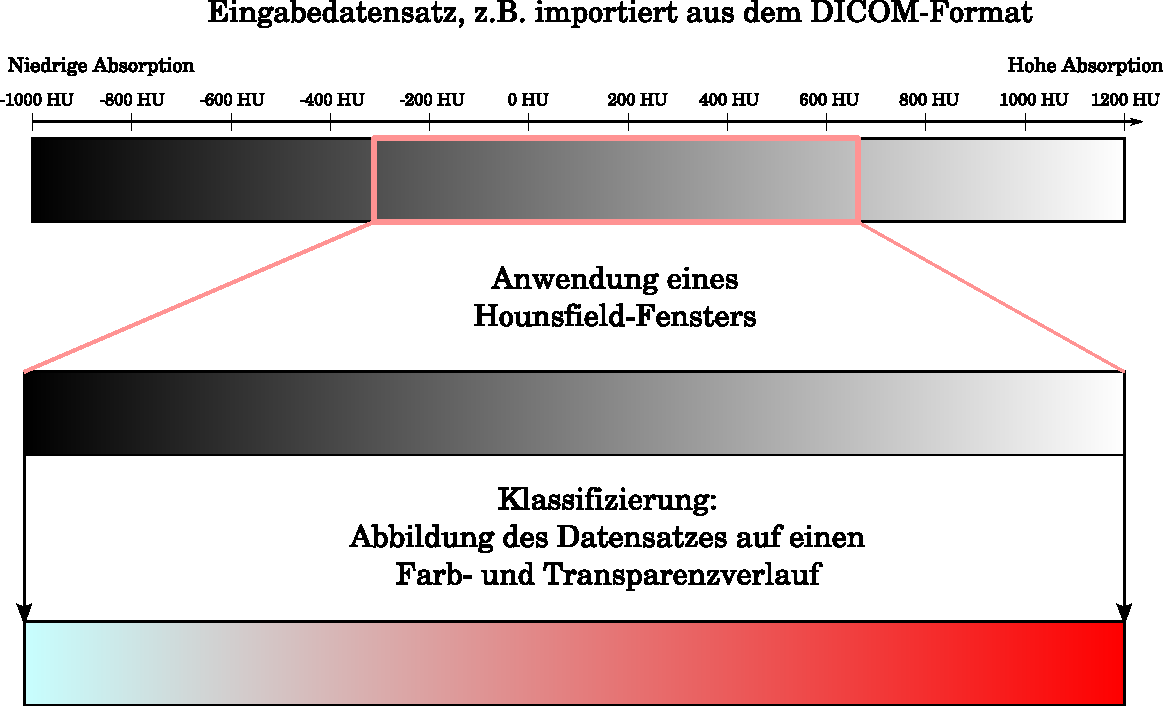
\includegraphics[width=\textwidth]{graphics/Classification.pdf}
\caption{Verarbeitung von CT-Eingabedaten in VERTEBRA}
\label{fig:gradientmapping-graphic}
\end{center}
\end{figure}\label{ssec:implementations}

\begin{figure}[p]
\begin{center}
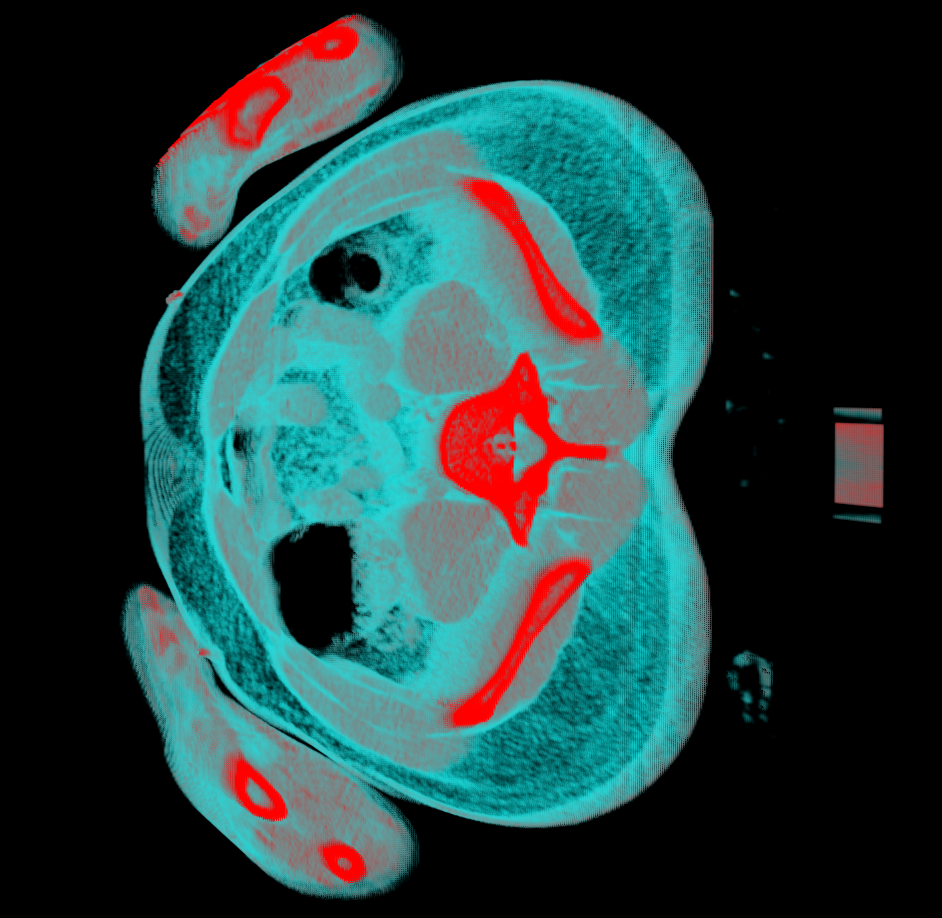
\includegraphics[width=\textwidth]{graphics/vertebra-screenshot-1.png}
\caption{Beispielrendering aus VERTEBRA}
\label{fig:vertebra-screenshot}
\end{center}
\end{figure}\label{ssec:implementations}

\section{Augmented Reality - Zukunft von Visualisationssystemen?}\label{sec:augmentedreality}
In den letzten Jahren wird neben den herkömmlichen Displays intensiv an der so genannten \glqq Augmented Reality\grqq\ geforscht. Dieser Begriff, der sich mit 'Erweiterte Realität' (Quelle: \cite[Seite 1]{Toe2010}) übersetzen lässt, beschreibt laut \cite{Suthau2002DE} (Seite 1; Englische Publikation: \cite{Suthau2002}) das Konzept, reale Bilder mit zusätzlichen Informationen zu ergänzen.

\subsection{Displays für Augmented Reality-Applikationen}\label{ssec:ardisplays}
In \cite[Kapitel 2.2, Seite 21]{Toe2010} werden zwei grundsätzliche Methoden unterschieden, die Kombination von realen und virtuellen Daten in Displays umzusetzen:
\begin{itemize}
 \item \textbf{Optical See-Through Displays}: Diese Art von Displays, ermöglicht den \glqq direkten Blick auf die umgebende Welt\grqq\footnoteremember{f:Toe2010-S21}{Zitiert aus \cite[Kapitel 2.2, Seite 21f.]{Toe2010}}. Technisch kann dieses Konzept beispielsweise durch einen halbdurchlässigen Spiegel, der Combiner genannt wird, realisiert werden. Dadurch bleibt die \glqq direkte Sicht auf die Umgebung\grqq\footnoterecall{f:Toe2010-S21} erhalten und die Darstellungsqualität der realen Informationen wird kaum verringert - lediglich der Transmissionsgrad des halbdurchlässigen Spiegels von mitunter weniger als 50\% führt zu einer verringerten Lichtstärke des realen Bildes (vgl. \cite[Kapitel 3.1.3, Seite 7]{Suthau2002DE}. Problematisch ist hierbei die je nach Geschwindigkeit des Systems verschieden große Verzögerung der virtuellen Komponente gegenüber dem realen Bild, die je nach Verarbeitung der Daten durch die Applikation unterschiedlich viel Zeit in Anspruch nehmen kann. Im Englischen wird diese Verzögerung mit \textit{lag} bezeichnet. Zur reinen Datenverarbeitung kommt hier noch hinzu, dass Position und Ausrichtung derjenigen Person, aus deren Sicht die Daten dargestellt werden sollen, von Sensoren erfasst und in Koordinaten und Winkel umgerechnet werden müssen, um dem Teil der Applikation, die die Visualisationsdaten berechnet, den zu rendernden Blickwinkel sowie die Position des Betrachters mitteilen zu können. (vgl. \cite[Kapitel 2.2, Seite 21f.]{Toe2010}). Eine zentrale Anforderung dieser Arbeit an die vorgestellten Konzepte ist, diesen \textit{lag} durch den Einsatz von echtzeitfähigen Algorithmen und Techniken gering zu halten - optimalerweise unter der Wahrnehmbarkeitsschwelle. Technisch bedingt ist diese Verzögerung jedoch immer vorhanden. Ein weiteres Problem von \textit{Optical See-Through Displays} stellt die Tatsache dar, dass durch die Projektion des virtuellen Bildes über den halbdurchlässigen Spiegel in jedem Fall das reale Umfeld des Betrachters durchscheint.
 \item \textbf{Video See-Through Displays}: Entgegen dem Ansatz von \textit{Optical See-Through Displays} wird bei diesen Displays das Bild komplett über einen bzw. (häufiger, siehe auch \glqq Head-Mounted Displays\grqq) zwei Monitore angezeigt. Der reale Anteil des Bildes wird hier über eine bzw. zwei Videokameras (je eine für jedes Auge) aufgenommen und um die gleiche Zeitspanne verzögert, die benötigt wird, um den virtuellen Anteil des Bildes soweit zu verarbeiten, dass er auf dem Monitor angezeigt werden kann. Durch das Fehlen eines halbdurchlässigen Spiegels kann konstruktionsbedingt für Teile des Bildes nur der virtuelle Anteil angezeigt werden.
 Obwohl bei dieser Art von Displays kein Unterschied zwischen dem \textit{lag} des realen und des virtuellen Bildes besteht, ist die Anzeige des Gesamtbildes verzögert. Zudem wird je nach Auflösung und Qualität der Kamera(s) beziehungsweise der Monitore der reale Anteil des Bildes in schlechterer Qualität als bei \textit{Optical See-Through Displays} dargestellt (vgl. \cite[Kapitel 2.2, Seite 22]{Toe2010}). 
\end{itemize}
Diese Konzepte werden zudem in \cite{Rolland2000} verglichen, wobei auch hier die technische Entwicklung seit des Erscheinens der Arbeit im Jahre 2000 berücksichtigt werden muss.

Basierend auf den dargestellten Grundkonzepten lassen sich laut \cite[Kapitel 2.2, Seite 22-30]{Toe2010} die folgenden Grundtypen von Displays unterscheiden, die in \cite{Toe2010} sowie in der einschlägigen Fachliteratur genauer erörtert werden:
 \begin{itemize}
 \item Head-Mounted Displays (HMDs); siehe \cite[Kapitel 2.2.1, Seite 23-25]{Toe2010}
 \begin{itemize}
  \item Monokulare Displays mit einem Bildschirm nur für ein Auge
  \item Binokulare Displays mit Bildschirmen für beide Augen
 \end{itemize}
 \item Raum- und umgebungsfixierte Displays; siehe \cite[Kapitel 2.2.2, Seite 25-28]{Toe2010}, darunter:
 \begin{itemize}
    \item Feststehende Displays
    \item Relativ feststehende Displays
 \end{itemize}
 \item Bewegliche Displays; siehe \cite[Kapitel 2.2.3, Seite 28]{Toe2010}
 \item Handheld-Displays; siehe \cite[Kapitel 2.2.4, Seite 28f.]{Toe2010}
 \item VRD (Virtual Retinal Display): Hierbei wird das Bild von Laserstrahlen direkt auf die Netzhaut projiziert; siehe \cite[Kapitel 3.1.2, Seite 5f.]{Suthau2002DE}
\end{itemize}

\subsubsection{Stereoskopische und Autostereoskopische Displays}
Bei den bereits genannten Displays lassen sich Displays, die nur eine zweidimensionale Sicht erlauben, von stereoskopischen Displays abgrenzen, die entweder durch spezielle Brillen (z.B. Shutterbrillen) oder durch autostereoskopische Verfahren, die keine solche Brille benötigen, dreidimensionale Bilder anzeigen. Binokulare HMDs sind prinzipbedingt stereoskopisch (vgl. \cite[Kapitel 2.2.1, Seite 23-25]{Toe2010}).

\subsubsection{Weitere Darstellungsmethoden}
Schlussendlich sei noch darauf hingewiesen, dass aufgrund der obigen Definition von Augmented Reality abgesehen von den bereits genannten Darstellungen durch visuelle Mittel auch die folgenden nicht visuellen Erweiterungen der Realität sowie Kombinationen möglich sind, die in \cite[Kapitel 2.4, Seite 36-41]{Toe2010} erörtert werden. 
\begin{itemize}
 \item Akustische Darstellung; siehe \cite[Seite 37]{Toe2010}
 \item Taktile bzw. haptische Darstellung; siehe \cite[Seite 38f.]{Toe2010}
 \item Gustatorische\footnote{Gustatorisch - Den Geschmackssinn betreffend} bzw. olfaktorische\footnote{Olfaktorisch - den Geruchssinn betreffend} Darstellung; siehe \cite[Seite 39-41]{Toe2010}
\end{itemize}

\section{ARION\texttrademark - Beispiel für ein existierendes Visualisationssystem}\label{sec:arion}
Wie bereits in Kapitel \vref{ssec:applications} beschrieben, existieren bereits jetzt für verschiedene Anwendungsbereiche innerhalb der Medizin verschiedene Visualisationssysteme. Da die Zahl der bestehenden Systeme unüberschaubar groß ist, soll an dieser Stelle exemplarisch das System ARION\texttrademark diskutiert werden, das sich auch für den Einsatz als Tumorvisualisationssystem eignet.

Das System ARION\texttrademark\textsuperscript{,}\footnote{ARION\texttrademark - Augmented Reality for Intra-Operative Navigation} wurde von der Abteilung für Medizinische und Biologische Informatik sowie der Chirurgischen und Radiologischen Klinik der Universität Heidelberg als Augmented Reality-basierender Prototyp eines intraoperativen Visualisationssystems (IGSS\footnote{IGSS - Image-guided surgery system - Bildgeführtes Operationssystem}) für die onkologische Leberchirurgie entwickelt. Suthau et al stellen in \cite{Suthau2002DE} bzw. \cite{Suthau2002} den Einsatz dieses Systems bei der Resektion eines Lebertumors dar. Die Autoren unterscheiden in \cite{Suthau2002DE} fünf Module des beschriebenen Einsatzes von ARION\texttrademark:
\begin{itemize}
 \item \textit{Modul 1}: Es wurden präoperativ kontrastmittelgestützte CT-Aufnahmen der betroffenen Leber angefertigt, anhand derer mithilfe des Operationsplanungssystem LENA des DKFZ\footnote{DKFZ - Deutsches KrebsForschungsZentrum} der chirurgische Eingriff geplant wurde. Zudem wurde hier ein mathematisches Modell (Graph) der Gefäße des betroffenen Organs erstellt.
 \item \textit{Modul 2}: Während des Eingriffs wurden mithilfe von Ultraschallaufnahmen die Gefäßbäume erfasst und ebenfalls dreidimensional als Graph modelliert. Während die Module 2 bis 4 ausgeführt werden, wird die betroffene Leber fixiert.
 \item \textit{Modul 3}: Die prä- und intraoperativen Gefäßgraphen, werden 
zueinander registriert\footnote{Registrierung - Prozess, der versucht, die beste Überlagerung zwischen zwei Graphen zu finden}; daher können mithilfe eines Trackingsystems die in der Planung festgelegten Schritte exakt ausgeführt werden.
 \item \textit{Modul 4}: Navigationshilfen werden in der Nähe des Tumors in die Leber eingesetzt, um während des Eingriffes Lageveränderungen mitverfolgen zu können und somit die geplanten Schritte auch weiterhin exakt ausführen zu können.
 \item \textit{Modul 5}: Während der Resektion werden auch die chirurgischen Instrumente mithilfe des zuvor beschriebenen Trackingsystems lokalisiert - diese Informationen werden \glqq in Beziehung zu den transparenten intrahepatischen\footnote{Intrahepatisch - Innerhalb der Leber liegend} Strukturen\grqq\footnote{Zitiert aus \cite[Kapitel 2, Seite 3]{Suthau2002DE}} gesetzt und auf einem Flachbildschirm angezeigt.
\end{itemize}

ARION erfüllt die in Kapitel \ref{ssec:requirements} dargestellten Anforderungen an ein Tumorvisualisationssystem: Die Interaktionsfähigkeit ist beispielsweise durch die Reaktion des Systems bei Änderung der chirurgischen Instrumente gegeben; der intraoperative Teil von ARION\texttrademark arbeitet soweit aus \cite{Suthau2002DE} ersichtlich in Echtzeit. Sowohl der präoperative  als auch der intraoperative Teil generiert aus medizinischen, dreidimensionalen Eingabedaten Ausgabedaten, die in ihrer Qualität ausreichend sind, um während einer realen Tumorresektion eingesetzt zu werden. Obwohl in \cite{Suthau2002DE} nicht explizit erwähnt, legt der Einssatzzweck nahe, dass ARION\texttrademark ein Klassifizierungsverfahren für Tumoren implementiert, da der Chirurg für eine erfolgreiche Resektion den Tumor auf dem Display erkennen können muss.

\section{Fazit und Ausblick}\label{sec:facit}
In dieser Arbeit wurden Konzepte und Methoden zur dreidimensionalen Visualisierung von Tumoren vorgestellt.
Der Vergleich von Software- und Hardwarealgorithmen in Kapitel \ref{ssec:swhwcomparison} sowie die behandelten Plattformen in Kapitel \ref{ssec:platforms} zeigten, dass bei der Auswahl der Plattform letztlich immer ein Kompromiss zwischen Kompatibilität und Geschwindigkeit gefunden werden muss, jedoch in der Forschung verschiedenste Ansätze verfolgt werden. Das vorgestellte exemplarische Konzept zur Tumorklassifizierung sowie die Proof-of-Concept-Implementierung VERTEBRA verdeutlichen, dass die Implementierung von einfachen, performanten Klassifizierungsverfahren ohne großen Aufwand möglich ist, jedoch prinzipbedingt alle Visualisationssysteme Grenzen haben.
Das in Kapitel \ref{sec:augmentedreality} vorgestellte Konzept der Augmented Reality zeigt einen der Einsatzbereiche der vorgestellten Algorithmen und Methoden, der Gegenstand vieler aktueller Forschungsprojekte ist. Zudem wurde mit ARION\texttrademark ein System vorgestellt, das auf Augmented Reality-Methoden basiert - dieses zeigte schon 2002, dass der Einsatz von Augmented Reality-basierenden Systemen für onkologische Operationen möglich ist. Durch eine weitere Verbesserung der Technik sowie der Algorithmen wird der Einsatz von medizinischen Visualisationssystemen, speziell auch von Tumorvisualisationssystemen in den nächsten Jahren weiter steigen.

\newpage
\appendix \label{appendixstart}
\section{Die Begleit-CD}
Dieser Arbeit liegt eine Begleit-CD, die die folgenden Daten enthält:
\begin{itemize}
 \item Quellcode von VERTEBRA im Verzeichnis \texttt{vertebra} sowie eine Anleitung zur Übersetzung in der Datei \texttt{INSTALL} in ebendiesem Verzeichnis
 \item Doxygen\footnote{Doxygen: Programm, um Dokumentationen aus Quellcode zu extrahieren}-Dokumentation von VERTEBRA als HTML sowie als PDF im Verzeichnis \texttt{doc}
 \item \LaTeX-Quellcode dieser Seminararbeit sowie die Arbeit als verlinkte PDF-Version\footnote{Für die digitale Version wurde das Paket \texttt{hyperref} benutzt, um durch Klicks innerhalb des Dokuments umherspringen zu können. Für die korrekte Verklinkung kann keine Gewähr übernommen werden} im Verzeichnis \texttt{latex} 
\end{itemize}

Hinweis: Alle Quellcodekommentare sowie Dokumentationen zu VERTEBRA wurden in englischer Sprache verfasst, da dies eine mögliche Weiterentwicklung des Projektes vereinfachen würde.

Zusätzlich liegt eine Sicherungskopie der Begleit-CD mit identischem Dateninhalt bei, die zur Absicherung gegen technische Defekte dient.

\section{Testplattform}\label{apdx:testplatform}
Die in dieser Arbeit vorgestellten Geschwindigkeitsmessungen wurden auf der folgenden Plattform durchgeführt:
\begin{itemize}
  \item Dell Inspiron 530
  \item CPU: Intel\textsuperscript{\textregistered} Core\texttrademark 2 Duo E8300; 2.83GHz Taktfrequenz
  \item Betriebssystem: KUbuntu 10.10 x86\_64; Kernel 2.6.35-22-generic x86\_64
  \item Grafikhardware: NVidia\textsuperscript{\textregistered} GeForce 9400 GT, PCI Express x16\\
	Treiber 260.19.06 (Konfiguration: High Performance)
\end{itemize}
\newpage
\section{Verzeichnisse}
%\nocite{*}
\listoffigures
\renewcommand\refname{Literatur- und Quellenverzeichnis}
\bibliographystyle{alphadin}
\bibliography{visualization}
\clearpage
\section{Selbstständigkeitserklärung}
Hiermit erkläre ich, dass ich die vorliegende Arbeit in allen Teilen selbstständig verfasst habe und keine anderen als die angegebenen Quellen und Hilfsmittel (einschließlich Onlinequellen und elektronischer Medien) benutzt habe. 
\vfill
\begin{center}
\underline{\hspace{10cm}}\vspace{1cm}
\end{center}
\begin{center}
Ulrich Köhler
\end{center}
\vfill
\end{document}
